\section{Experimental Validation}

In an attempt to show that the model works, I created the program

\begin{figure}[H]
    \centering
    % 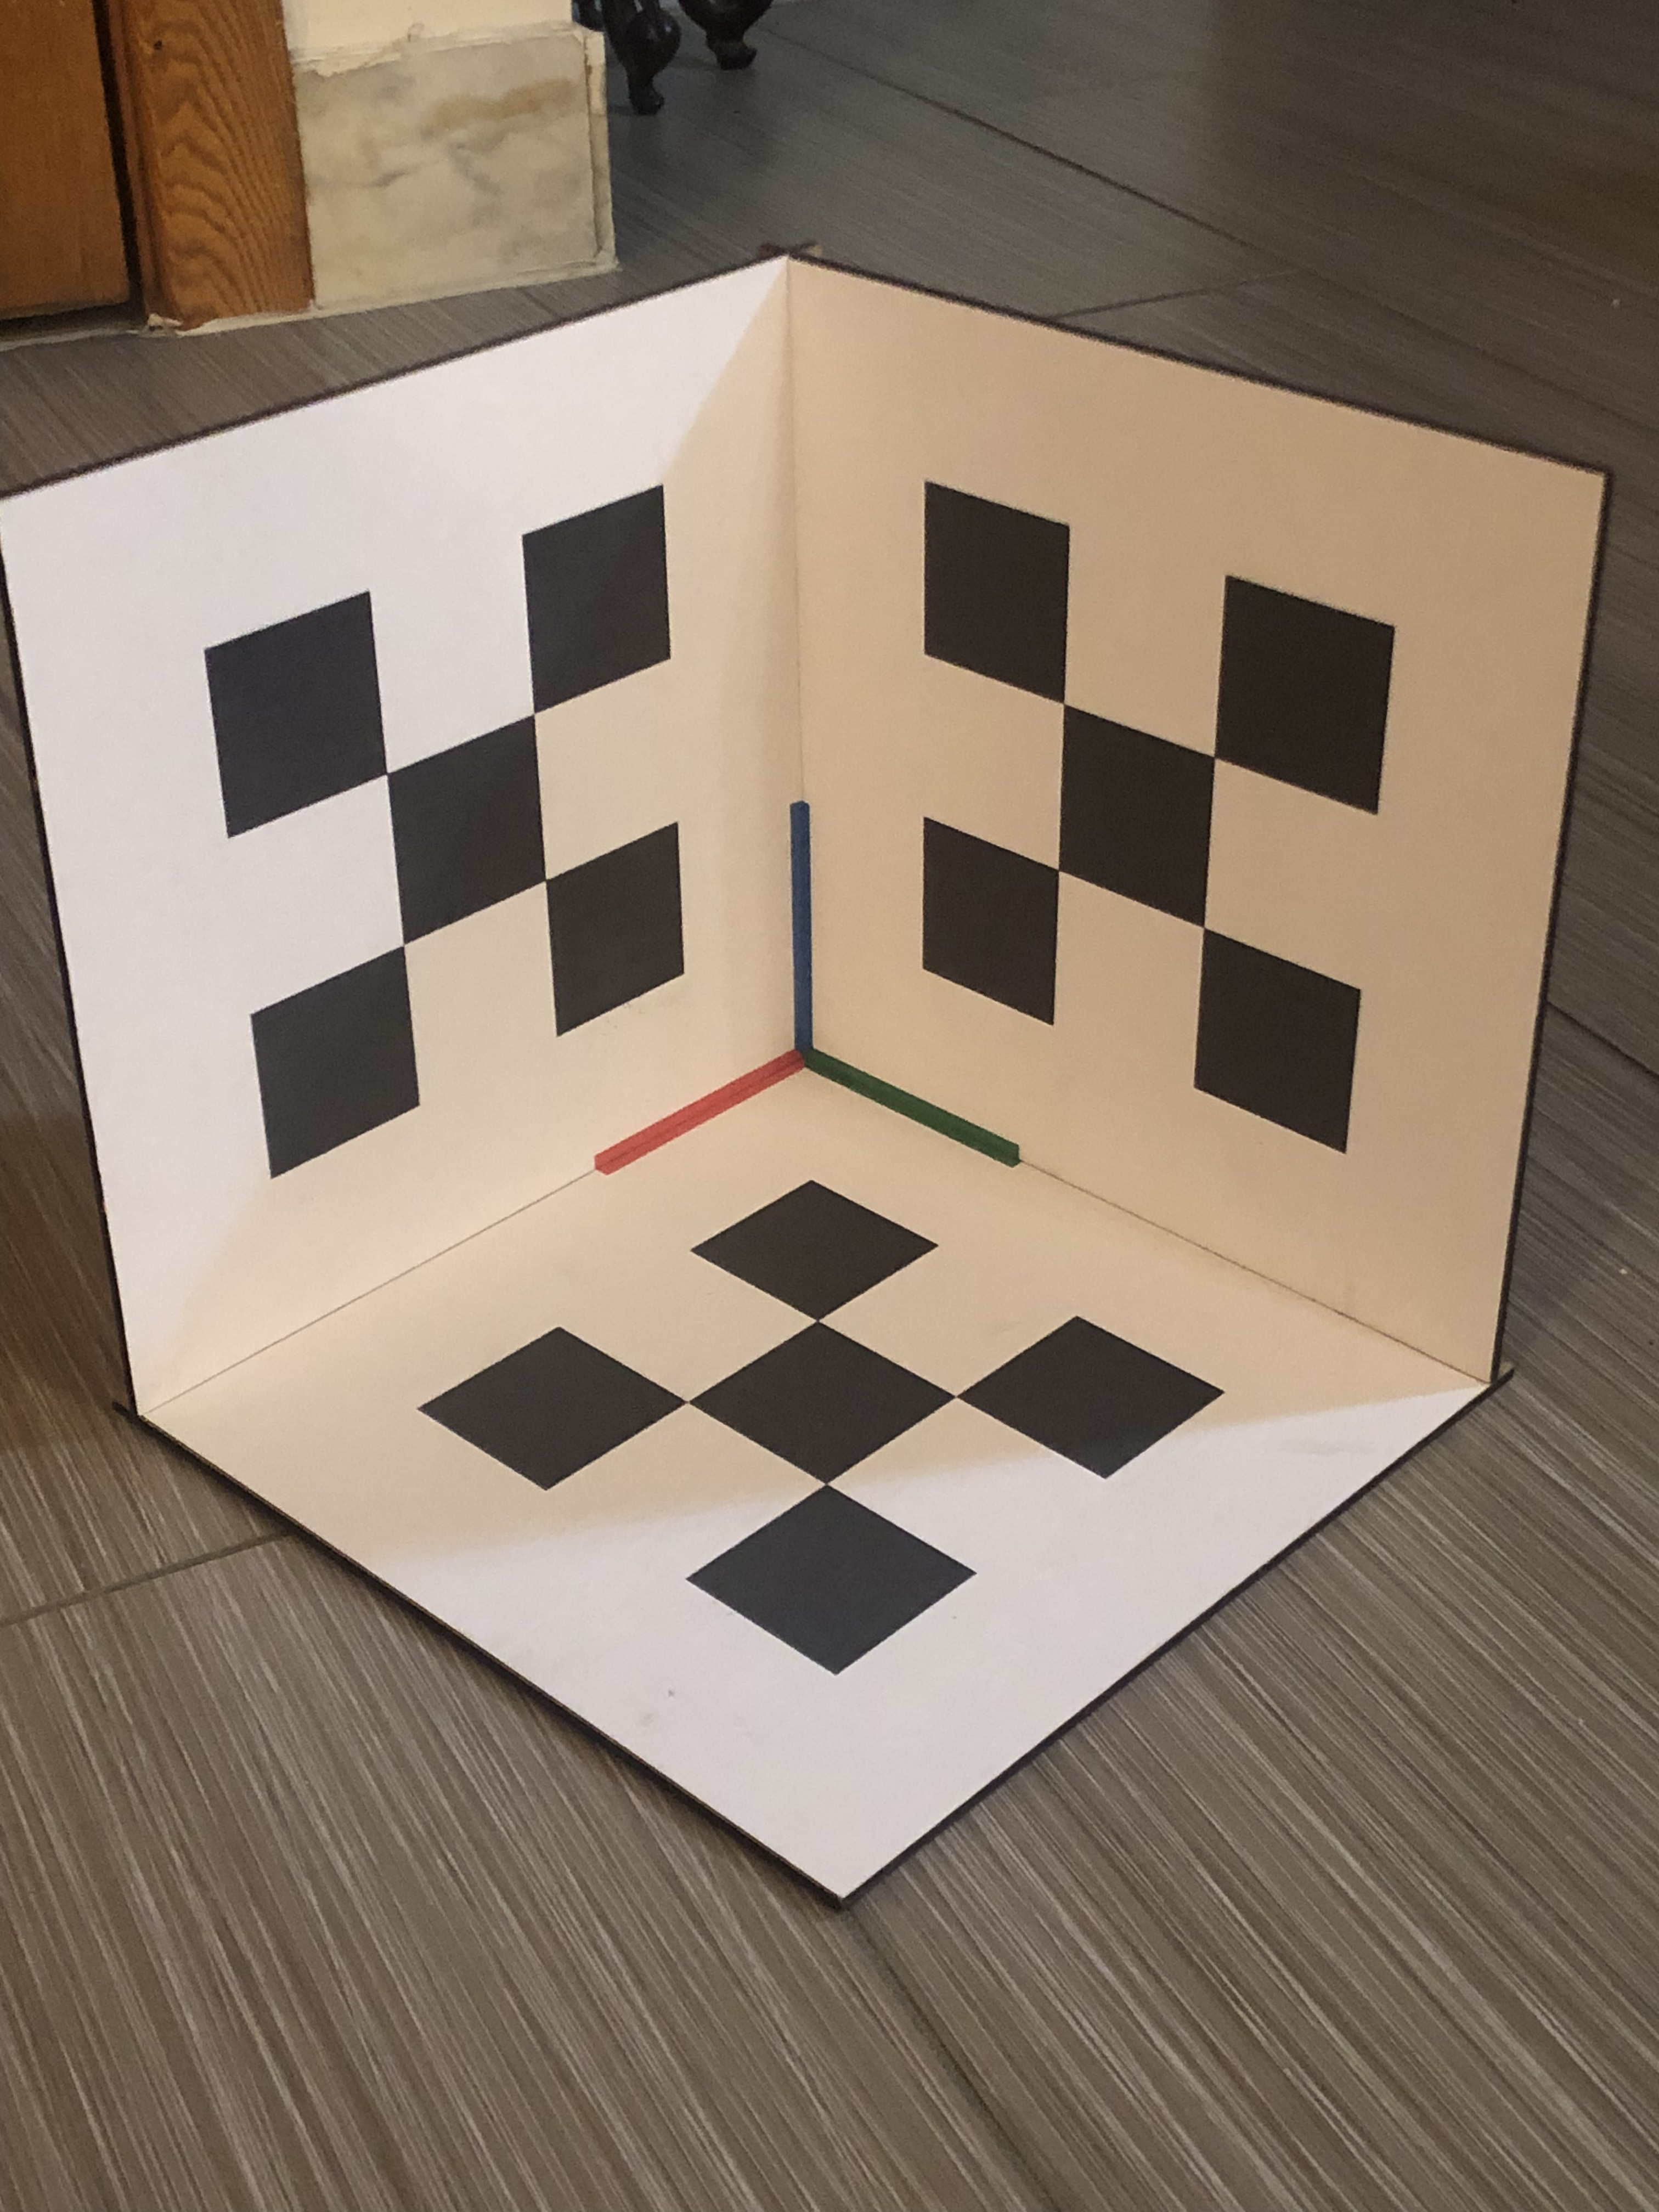
\includegraphics[width=0.45\textwidth]{assets/images/iphone_image}
    \caption{Photograph 1. The photo editing software \emph{GIMP} was used for edge detection, and the coordinates of the calibration points were selected manually. }
\end{figure}



\begin{figure}[H]
    \centering
    % \includegraphics[width=0.6\textwidth]{assets/graphs/iphone_graph}
    \caption{Graph produced by \texttt{Matplotlib} which displays the results of the trial}
\end{figure}

\begin{equation*}
    P =
    \begin{bmatrix}
        \num{-2.5844e-03} & \num{1.7334e-03}  & \num{-4.6719e-04} & \num{6.0581e-01} \\
        \num{4.8240e-04}  & \num{4.4097e-04}  & \num{-3.1337e-03} & \num{7.9559e-01} \\
        \num{-3.3990e-07} & \num{-3.1311e-07} & \num{-2.8179e-07} & \num{4.1340e-04}
    \end{bmatrix}
\end{equation*}

\begin{table}
    \begin{tabular}{p{3cm}cccc}
    \toprule
                                                     &             & \textbf{\small Canon EOS D80} & \textbf{\small IPhone X} & \textbf{\small Nikon D100} \\
    \midrule
    \addlinespace
    \multirow{2}{*}{\footnotesize Focal Lengths}     & $f_x$       & $\qty{8404.1}{\pixel}$        & $\qty{3281.5}{\pixel}$   & $\qty{8144.4}{\pixel}$     \\
                                                     & $f_y$       & $\qty{8387.9}{\pixel}$        & $\qty{3279.9}{\pixel}$   & $\qty{8142.6}{\pixel}$     \\
    \addlinespace
    \multirow{2}{*}{\footnotesize Principal Point}   & $c_x$       & $\qty{3151.6}{\pixel}$        & $\qty{2043.0}{\pixel}$   & $\qty{1541.8}{\pixel}$     \\
                                                     & $c_y$       & $\qty{1972.8}{\pixel}$        & $\qty{1453.1}{\pixel}$   & $\qty{1027.9}{\pixel}$     \\
    \addlinespace
    \midrule
    \addlinespace
    \multirow{3}{*}{\footnotesize Tait-Bryan Angles} & $\alpha$    & $\qty{-81.86}{\degree}$       & $\qty{-60.21}{\degree}$  & $\qty{-70.83}{\degree}$    \\
                                                     & $\beta$     & $\qty{44.27}{\degree}$        & $\qty{38.72}{\degree}$   & $\qty{46.44}{\degree}$     \\
                                                     & $\gamma$    & $\qty{4.97}{\degree}$         & $\qty{21.64}{\degree}$   & $\qty{13.89}{\degree}$     \\
    \addlinespace
    \multirow{3}{*}{\footnotesize Translation}       & $t_x$       & $\qty{494.8}{\mm}$            & $\qty{329.0}{\mm}$       & $\qty{840.3}{\mm}$         \\
                                                     & $t_y$       & $\qty{537.6}{\mm}$            & $\qty{321.4}{\mm}$       & $\qty{766.0}{\mm}$         \\
                                                     & $t_z$       & $\qty{128.3}{\mm}$            & $\qty{208.6}{\mm}$       & $\qty{317.2}{\mm}$         \\
    \addlinespace
    \midrule
    \addlinespace
    \multirow{2}{*}{\footnotesize Reproj. Errors}    & $\mu_{max}$ & $\qty{11.08}{\pixel}$         & $\qty{5.58}{\pixel}$     & $\qty{11.70}{\pixel}$      \\
                                                     & $\mu_{avg}$ & $\qty{3.56}{\pixel}$          & $\qty{2.55}{\pixel}$     & $\qty{2.81}{\pixel}$       \\
    \addlinespace
    \bottomrule
\end{tabular}



 
    \caption{Intrinsic and Extrinsic Parameters calculated by \texttt{calicam}.}
\end{table}


